\begin{frame}{Graphs and \msts\ in \dpm: Underlying forest and \mst\ (I)}
    \begin{definition}\label{def:u-forest}
        Given a graph $G=(V,E)$, we say that the sequence $F_G = \langle T_1,\dots,T_k\rangle$, $k \ge 1$, 
        is an \emph{underlying forest} of $G$ 
        if $T_i \subseteq E$ $\forall i$, $\cup_{i=1}^k T_i = E$, $\forall i,j, i\neq j, T_i\cap T_j = \emptyset$
        and  $\forall i\:\: T_i\in F_G$ there exists a distinguished vertex $v_i\in V$, called the \emph{root} 
        of $T_i$, such that $\forall e \in T_i$,  $e$ is incident to $v_i$.
    \end{definition}

    \textcolor{white}{Here goes some text}
    
    \resizebox{\textwidth}{!}{
    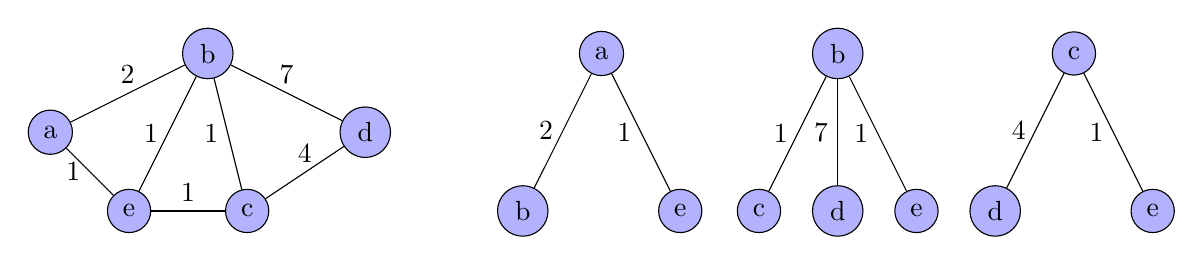
\begin{tikzpicture}
        \node[shape=circle,draw=black, fill = blue!30] (a) at (-3,0) {a};
        \node[shape=circle,draw=black, fill = blue!30] (b) at (-1,1) {b};
        \node[shape=circle,draw=black, fill = blue!30] (c) at (-0.5,-1) {c};
        \node[shape=circle,draw=black, fill = blue!30] (d) at (1,0) {d};
        \node[shape=circle,draw=black, fill = blue!30] (e) at (-2,-1) {e};
    
        \path [-] (a) edge node[above] {$2$} (b);
        \path [-](a) edge node[left] {$1$} (e);
        \path [-](b) edge node[left] {$1$} (e);
        \path [-](b) edge node[left] {$1$} (c);
        \path [-](b) edge node[above] {$7$} (d);
        \path [-](c) edge node[above] {$4$} (d);
        \path [-](e) edge node[above] {$1$} (c);  
    
        \node[shape=circle,draw=black, fill = blue!30] (f) at (4,1) {a};
        \node[shape=circle,draw=black, fill = blue!30] (g) at (3,-1) {b};
        \node[shape=circle,draw=black, fill = blue!30] (h) at (5,-1) {e};
      
        \path [-] (f) edge node[left] {$2$} (g);
        \path [-](f) edge node[left] {$1$} (h);
    
        \node[shape=circle,draw=black, fill = blue!30] (i) at (7,1) {b};
        \node[shape=circle,draw=black, fill = blue!30] (j) at (6,-1) {c};
        \node[shape=circle,draw=black, fill = blue!30] (k) at (7,-1) {d};
        \node[shape=circle,draw=black, fill = blue!30] (l) at (8,-1) {e};
      
        \path [-] (i) edge node[left] {$1$} (j);
        \path [-](i) edge node[left] {$7$} (k);
        \path [-](i) edge node[left] {$1$} (l);
    
        \node[shape=circle,draw=black, fill = blue!30] (m) at (10,1) {c};
        \node[shape=circle,draw=black, fill = blue!30] (n) at (9,-1) {d};
        \node[shape=circle,draw=black, fill = blue!30] (o) at (11,-1) {e};
      
        \path [-] (m) edge node[left] {$4$} (n);
        \path [-](m) edge node[left] {$1$} (o);
    \end{tikzpicture}
    }
\end{frame}

\begin{frame}{Graphs and \msts\ in \dpm: Underlying forest and \mst\ (II)}
        \begin{proposition}
        Given a weighted graph $G=(V,E)$ represented by the underlying forest 
        $F_G = \langle T_1, \dots, T_k\rangle\ (k \ge 1)$ and the subgraphs $G_i$, $1\leq i\leq k$, of $G$ 
        such that $G_i = \cup_{j=1}^kT_i$, it holds that
            \[
                \mathsf{MST}(G_i) =     \left\{ \begin{array}{lr}
        				                    T_1& \mbox{if}\:\: i = 1 \\ 
        				                    \mathsf{MST}(T_i \cup \mathsf{MST}(G_{i-1})) & \mbox{if}\:\: i > 1 \\
        			                \end{array}\right.
            \]
        where \mst(G) is any correct procedure to compute a \mst\ of $G$.
    \end{proposition}
\end{frame}

\begin{frame}{Graphs and \msts\ in \dpm: Stages of Dynamic Pipeline}
    \begin{itemize}
        \item<2-> \textbf{Source:} This stage manages the in-connection with the outside: streaming input, file reading, random generation...
        \item<3-> \textbf{Sink:} This stage manages the out-connection. Usually stdout
        \item<4-> \textbf{Generator:} If operation requires to be processed by a filter, it will generate a new filter.
        \item<5-> \textbf{Filter:} This (statefull) stage will select which operations to perform and wich ones have to be passed to the next filter. It will do the main work.
    \end{itemize}
    
    \centering
    \begin{tikzpicture}
        \begin{pgfonlayer}{nodelayer}
            \node [style=io, minimum height=1.25cm, minimum width=3.5cm, shape border rotate=270, visible on=<2->] (0) at (-3, 0) {Source};
            \node [style=filter_gen, minimum width=1cm, minimum height=2.5cm, visible on=<5->] (1) at (-1, 0) {Filter};
            \node [style=filter_gen, minimum width=1cm, minimum height=2.5cm, visible on=<5->] (2) at (0.9, 0) {Filter};
            \node [style=filter_gen, minimum width=1cm, minimum height=2.5cm, align=center, visible on=<4->] (3) at (3.2, 0) {Generator \\ 
\includegraphics[width=.05\textwidth]{gear} };
            \node [style=io, minimum height=1.25cm, minimum width=3.5cm, shape border rotate=90, visible on=<3->] (4) at (5.7, 0) {Sink};
        \end{pgfonlayer}
        \begin{pgfonlayer}{edgelayer}
            \draw [style={opChan}, visible on=<6->] ([yshift=0.5 cm]0.east) to["Op"] ([yshift=0.5 cm]1.west);
            \draw [style={opChan}, visible on=<6->] ([yshift=0.5 cm]1.east) to["Op"] ([yshift=0.5 cm]2.west);
            \draw [style={opChan}, visible on=<6->] ([yshift=0.5 cm]2.east) to["Op"] ([yshift=0.5 cm]3.west);
            \draw [style={opChan}, visible on=<6->] ([yshift=0.5 cm]3.east) to["Op"] ([yshift=0.5 cm]4.west);
            
            \draw [style={daChan}, visible on=<6->] ([yshift=-0.5 cm]0.east) to["Data"] ([yshift=-0.5 cm]1.west);
            \draw [style={daChan}, visible on=<6->] ([yshift=-0.5 cm]1.east) to["Data"] ([yshift=-0.5 cm]2.west);
            \draw [style={daChan, visible on=<6->}] ([yshift=-0.5 cm]2.east) to["Data"] ([yshift=-0.5 cm]3.west);
            \draw [style={daChan}, visible on=<6->] ([yshift=-0.5 cm]3.east) to["Data"] ([yshift=-0.5 cm]4.west);
        \end{pgfonlayer}
    \end{tikzpicture}
\end{frame}

\begin{frame}{Graphs and \msts\ in \dpm: \DPmst}
    \begin{center}
    \resizebox{1\textwidth}{!}{
    \begin{tikzpicture}
        \begin{pgfonlayer}{nodelayer}
            \node [style=io, minimum height=0.8cm, minimum width=3cm, shape border rotate=270] (In) at (0, 0) {I};
            \node [style=filter_gen, minimum width=1.5cm, minimum height=2.5cm, right= 1cm of In,  text depth = 1cm] (F1) {$F_a$};
            \node [style=filter_gen, minimum width=1.5cm, minimum height=2.5cm, right= 1cm of F1,  text depth = 1cm] (F2) {$F_c$};
            \node [style=filter_gen, minimum width=1.5cm, minimum height=2.5cm, right= 1cm of F2,  text depth = 1cm] (F3) {$F_d$};
            \node [style=filter_gen, minimum width=0.8cm, minimum height=2.5cm, align=center, right= 1cm of F3] (Gen) {Gen};
            \node [style=io, minimum height=0.8cm, minimum width=3.2cm, shape border rotate=90, right= 1cm of Gen] (Out) {O};
        \end{pgfonlayer}
        \begin{pgfonlayer}{edgelayer}
                \draw [style={opChan}] ([yshift=0.5 cm]Gen.east) to["Op"] ([yshift=0.5 cm]Out.west);
                \draw [style={daChan}] ([yshift=-0.5 cm]Gen.east) to["\mst\ "] ([yshift=-0.5 cm]Out.west);

                \draw [style={opChan}] ([yshift=0.5 cm]In.east) to["Op"] ([yshift=0.5 cm]F1.west);
                \draw [style={daChan}] ([yshift=-0.5 cm]In.east) to["\mst\ "] ([yshift=-0.5 cm]F1.west);
                
                \draw [style={opChan}] ([yshift=0.5 cm]F1.east) to["Op"] ([yshift=0.5 cm]F2.west);
                \draw [style={daChan}] ([yshift=-0.5 cm]F1.east) to["\mst\ "] ([yshift=-0.5 cm]F2.west);
                
                \draw [style={opChan}] ([yshift=0.5 cm]F2.east) to["Op"] ([yshift=0.5 cm]F3.west);
                \draw [style={daChan}] ([yshift=-0.5 cm]F2.east) to["\mst\ "] ([yshift=-0.5 cm]F3.west);
                \draw [style={opChan}] ([yshift=0.5 cm]F3.east) to["Op"] ([yshift=0.5 cm]Gen.west);
                \draw [style={daChan}] ([yshift=-0.5 cm]F3.east) to["\mst\ "] ([yshift=-0.5 cm]Gen.west);
        \end{pgfonlayer}

        \begin{pgfonlayer}{embeded}
            %Filter 1
            \node [style=new style 0, scale=0.5] (a1) at (2.17, -0.1) {a};
            \node [style=new style 0, scale=0.5,below=0.18cm of a1] (b1) {b};
            \node [style=new style 0, scale=0.5,below left=0.4cm of a1] (c1) {c};
            \node [style=new style 0, scale=0.5,below right=0.4cm of a1] (d1) {d};
            \draw[style={tree_edge}]{} (a1) to (b1);
            \draw[style={tree_edge}]{} (a1) to (c1);
            \draw[style={tree_edge}]{} (a1) to (d1);
            
            %Filter 2
            \node [style=new style 0, scale=0.5] (c2) at (4.72, -0.1) {c};
            \node [style=new style 0, scale=0.5,below left=0.4cm of c2] (d2) {d};
            \node [style=new style 0, scale=0.5,below right=0.4cm of c2] (e2) {e};
            \draw[style={tree_edge}]{} (c2) to (d2);
            \draw[style={tree_edge}]{} (c2) to (e2);
            
            %Filter 3
            \node [style=new style 0, scale=0.5] (d3) at (7.27, -0.1) {d};
            \node [style=new style 0, scale=0.5,below=0.18cm of d3] (f3) {f};
            \draw[style={tree_edge}]{} (d3) to (f3);
        \end{pgfonlayer}
    \end{tikzpicture}
    }
    \end{center}

    \resizebox{0.9\textwidth}{!}{
    %Input MST
    \begin{tikzpicture}
        \begin{pgfonlayer}{nodelayer}
            \node[style=new style 0] (a) at (0,0) {a};
            \node[style=new style 0, left=1cm of a] (b) {b};
            \node[style=new style 0, above right=1.118cm of a] (c) {c};
            \node[style=new style 0, below right=1.118cm of a] (d) {d};
            \node[style=new style 0, right=1cm of c] (e) {e};
            \node[style=new style 0, right=1cm of d] (f) {f};
        \end{pgfonlayer}
        \begin{pgfonlayer}{edgelayer}
            \draw[style={tree_edge}]{} (b) to["0.4"] (a);
            \draw[style={tree_edge}]{} (c) to["0.3"] (d);
            \draw[style={tree_edge}]{} (a) to["0.6"] (c);
            \draw[style={tree_edge}]{} (d) to["0.1"] (f);
            \draw[style={tree_edge}]{} (d) to["0.8"] (a);
            \draw[style={tree_edge}]{} (c) to["0.9"] (e);
        \end{pgfonlayer}
    \end{tikzpicture}
    
    %Output MST
    \begin{tikzpicture}
        \begin{pgfonlayer}{nodelayer}
            \node[style=new style 0] (a) at (0,0) {a};
            \node[style=new style 0, left=1cm of a] (b) {b};
            \node[style=new style 0, above right=1.118cm of a] (c) {c};
            \node[style=new style 0, below right=1.118cm of a] (d) {d};
            \node[style=new style 0, right=1cm of c] (e) {e};
            \node[style=new style 0, right=1cm of d] (f) {f};
        \end{pgfonlayer}
        \begin{pgfonlayer}{edgelayer}
            \draw[style={tree_edge}]{} (b) to["0.4"] (a);
            \draw[style={tree_edge}]{} (c) to["0.3"] (d);
            \draw[style={tree_edge}]{} (a) to["0.6"] (c);
            \draw[style={tree_edge}]{} (d) to["0.1"] (f);
            \draw[style={tree_edge}]{} (c) to["0.9"] (e);
        \end{pgfonlayer}
    \end{tikzpicture}
    }    
    
\end{frame}


\begin{frame}{Graphs and \msts\ in \dpm: \DPmst}
            \centering
            \begin{tikzpicture}                
                \node [style=filter_gen, minimum width=2.75cm, minimum height=3.5cm,  text depth = 2cm] (Fi) at (0.0, 0.0) {\LARGE $F_i$};

                \node [ left=2cm of Fi] (prev) {};
                \node [right=2cm of Fi] (post) {};

                % Input channels
                \draw [style={opChan}] ([yshift=0.75 cm]prev.east) to["Op"] ([yshift=0.75 cm]Fi.west);
                \draw [style={daChan}] ([yshift=-0.75 cm]prev.east) to["\mst($G_{i-1}$)"] ([yshift=-0.75 cm]Fi.west);

                % Output channels
                \draw [style={opChan}] ([yshift=0.75 cm]Fi.east) to["Op"] ([yshift=0.75 cm]post.west);
                \draw [style={daChan}] ([yshift=-0.75 cm]Fi.east) to["\mst($G_i$)"] ([yshift=-0.75 cm]post.west);

                % Embedded graph            
                \node [style=new style 0, scale=1] (a1) at (0, 0) {v};
                \node [scale=1,below=0.18cm of a1] (b1) {...};
                \node [style=new style 0, scale=1,below left=0.4cm of a1] (c1) {u};
                \node [style=new style 0, scale=1,below right=0.4cm of a1] (d1) {w};
                %\draw[style={tree_edge}]{} (a1) to (b1);
                \draw[style={tree_edge}]{} (a1) to (c1);
                \draw[style={tree_edge}]{} (a1) to (d1);
            \end{tikzpicture}
            
            \[
                \mathsf{MST}(G_i) = \left\{ \begin{array}{lr}
                                            T_1& \mbox{if}\:\: i = 1 \\ 
                                            \mathsf{MST}(T_i \cup \mathsf{MST}(G_{i-1})) & \mbox{if}\:\: i > 1 \\
                                    \end{array}\right.
            \]

            $\mathsf{MST}(T_i \cup \mathsf{MST}(G_{i-1}))$ is computed using \texttt{Kruskal}.
\end{frame}